\documentclass[a4paper]{jsarticle}
\setlength{\topmargin}{-20.4cm}
\setlength{\oddsidemargin}{-10.4mm}
\setlength{\evensidemargin}{-10.4mm}
\setlength{\textwidth}{18cm}
\setlength{\textheight}{26cm}

\usepackage[top=15truemm,bottom=25truemm,left=20truemm,right=20truemm]{geometry}
\usepackage[latin1]{inputenc}
\usepackage{amsmath}
\usepackage{amsfonts}
\usepackage{amssymb}
\usepackage[dvipdfmx]{graphicx}
\usepackage[dvipdfmx]{color}
\usepackage{listings}
\usepackage{listings,jvlisting}
\usepackage{geometry}
\usepackage{framed}
\usepackage{color}
\usepackage[dvipdfmx]{hyperref}
\usepackage{ascmac}
\usepackage{enumerate}
\usepackage{tabularx}

\renewcommand{\figurename}{fig.}
\renewcommand{\tablename}{table }

\hypersetup{
	colorlinks=false, % リンクに色をつけない設定
	bookmarks=true, % 以下ブックマークに関する設定
	bookmarksnumbered=true,
	pdfborder={0 0 0},
	bookmarkstype=toc
}

\lstset{
basicstyle={\ttfamily},
identifierstyle={\small},
commentstyle={\smallitshape},
keywordstyle={\small\bfseries},
ndkeywordstyle={\small},
stringstyle={\small\ttfamily},
frame={tb},
breaklines=true,
columns=[l]{fullflexible},
xrightmargin=0zw,
xleftmargin=3zw,
numberstyle={\scriptsize},
stepnumber=1,
numbersep=1zw,
lineskip=-0.5ex
}



\author{}
\title{大学院入試対策}
\date{}

\begin{document}
\maketitle

\section{基本知識}
\subsection{平方根}
$\sqrt{a^2}=|a|$
\subsection{オイラーの公式}
\begin{itembox}[l]{オイラーの公式}
    \begin{center}
        $e^{i\theta}=\cos\theta+i\sin\theta$
    \end{center}
\end{itembox}
\newpage
\section{線形代数}
\subsection{行列}
\subsubsection{行列演算の性質}
基本的には、普通の計算と同じ。
ただし、\textgt{積}には注意が必要。
\begin{itembox}[l]{行列演算特有の性質}
    \begin{eqnarray*}
        \left(AB\right)C&=&A\left(BC\right)\\
        A\left(B+C\right)&=&AB+AC\\
        \left(A+B\right)&=&AC+BC\\
        AB&\neq& BA
    \end{eqnarray*}
    ※ 積をとる順番に注意する\\
    ※ 積の交換法則のみ成り立たない!!
\end{itembox}
\subsection{一次独立・一次従属}
\begin{itembox}[l]{物理的な意味}
    ある2つのベクトル$a,b\left(a\neq 0,b\neq 0\right)$が存在し、
    それらが並行でない$\left(a\not\parallel b\right)$とき、\textgt{一次独立である}という。\\
    また、それらが、平行である$\left(a\parallel b\right)$とき、\textgt{一次従属である}という。
\end{itembox}
\subsection{連立一次方程式}
\subsubsection{行列の基本変形}
\begin{enumerate}[(1)]
    \item 1つの行を何倍か($\neq0$倍)する
    \item 2つの行を入れ替える
    \item 1つの行にほかの行の何倍かを加える
\end{enumerate}
\subsubsection{連立一次方程式の消去法による解法}
\begin{enumerate}[(1)]
    \item 連立一次方程式より拡大係数行列を抽出(行列のデータ化)
    \item 抽出した拡大係数行列を簡約化する(未知数の整理)
    \item 簡約化の結果を連立一次方程式に還元し解を作成する
\end{enumerate}
\subsubsection{解が不定の場合}
「1式に1未知数」という形は,一般には成り立たない.そこで,「1式に1未知数」に近い形に整理したものが\textgt{階段行列(=簡約行列)}である.
一般の連立1次方程式の場合,未知数,方程式の本数,任意定数の間には以下の関係が成り立つ.
\begin{center}
    \textgt{(未知数の個数) = (有効な方程式の数) + (任意定数の数)}
\end{center}
\subsubsection{単位行列}
\begin{itembox}[l]{定義}
    \begin{center}
        $E=
            \begin{bmatrix}
                1      & 0      & \cdots & 0      \\
                0      & 1      & \cdots & 0      \\
                \vdots & \vdots & \ddots & \vdots \\
                0      & 0      & \cdots & 1      \\
            \end{bmatrix}
            \quad AE=EA=A
        $
        \quad(対角成分は$1$、他は$0$)
    \end{center}
\end{itembox}
\subsubsection{逆行列}
\begin{itembox}[l]{定義}
    $n$次正方行列$A$に対して、
    \begin{center}
        $AX=XA=E$
    \end{center}
    となる正方行列$X$が存在するとき、$A$は\textgt{正則である}といい、$X$を$A$の\textgt{逆行列}であるという.\\
    一般に「$X$」を「$A^{-1}$」という記号で表す.\\
    ※「正則である」=「逆行列を持つ」という意味
\end{itembox}
\begin{itembox}[l]{定理}
    $n$次正方行列$A$が正則であるとき、その逆行列$A^{-1}$は、以下のように表せる。
    \begin{center}
        $A^{-1}=\dfrac{1}{|A|}\tilde{A}$
    \end{center}
    ※ $\tilde{A}$は余因子行列
\end{itembox}
\\
$n$次正方行列$A$が正則であるとは\dots
\begin{enumerate}[(1)]
    \item rank$\left(A\right)=n$\quad すなわち、\textgt{連立方程式の解が一意に定まる}ということ!!
    \item $\left|A\right|\neq0$
\end{enumerate}
\subsubsection{逆行列の掃出法}
$AX=E$\quad を満たす、$x$を求めれば、それが$A^{-1}$になる。
\begin{eqnarray*}
    X&=&\left(x_1,x_2,\cdots,x_n\right)\\
    E&=&\left(e_1,e_2,\cdots,e_n\right)
\end{eqnarray*}
※$x_i$ : $n$次元列ベクトル\quad $e_i$ : $n$次元単位ベクトル\\
を用いて、
\begin{eqnarray*}
    A\left(x_1,x_2,\cdots,x_n\right)&=&\left(e_1,e_2,\cdots,e_n\right)\\
    \left(Ax_1,Ax_2,\cdots,Ax_n\right)&=&\left(e_1,e_2,\cdots,e_n\right)
\end{eqnarray*}
すなわち、以下の式を解けばよい。
\begin{eqnarray*}
    Ax_i=e_i \left(i=1,2,\cdots,n\right)
\end{eqnarray*}
ここで、拡大係数行列を考える.
\begin{eqnarray*}
    \left(A|e_i\right) \rightarrow \left(E|C_i\right)
\end{eqnarray*}
上記のように掃出法から連立方程式を解くと、
\begin{eqnarray*}
    X=\left(x_1,x_2,\cdots,x_n\right)=\left(C_1,C_2,\cdots,C_n\right)
\end{eqnarray*}
が求める$A^{-1}$となる。
\subsection{行列式}
\subsubsection{行列式の性質}
※ 同じ行(列)を含む行列式の値$0$になる。(行列式の交代性より)
\subsubsection{余因子行列とクラメールの公式}
$n$次正方行列$A=\left[a_{ij}\right]$の第$i$行と第$j$列を取り除いて得られる
$n-1$次正方行列\textgt{(小行列)}を$A_{ij}$とする.
\begin{itembox}[l]{余因子行列}
    $n$次正方行列$\left[a_{ij}\right]$に対し,以下の式から得られる値$\tilde{a}_{ij}$を
    \textgt{余因子}という。
    \begin{center}
        $\tilde{a}_{ij}=\left(-1\right)^{i+j}\left|A_{ij}\right|$
    \end{center}
    さらに,以下のように余因子をおいた行列$\tilde{A}$を,$A$の\textgt{余因子行列}という.(転置があることに注意!!)
    \begin{center}
        $\tilde{A}=\left[\tilde{a}_{ij}\right]^t$
    \end{center}
    ※ 「転置をとる」とは、「添え字の順番が逆になる」ということ!!
\end{itembox}
\begin{itembox}[l]{余因子展開}
    \begin{enumerate}[(1)]
        \item 第$i$行に関する余因子展開\\
              $\left|A\right|=(-1)^{i+1}a_{i1}\left|A_{i1}\right|+(-1)^{i+2}a_{i2}\left|A_{i2}\right|+ \dots +(-1)^{i+n}a_{in}\left|A_{in}\right|
                  =a_{i1}\tilde{a}_{i1}+a_{i2}\tilde{a}_{i2}+\cdots +a_{in}\tilde{a}_{in}$
        \item 第$j$列に関する余因子展開\\
              $\left|A\right|=(-1)^{1+j}a_{1j}\left|A_{1j}\right|+(-1)^{2+j}a_{2j}\left|A_{2j}\right|+ \dots +(-1)^{n+j}a_{nj}\left|A_{nj}\right|
                  =a_{1j}\tilde{a}_{1j}+a_{2j}\tilde{a}_{2j}+\cdots +a_{nj}\tilde{a}_{nj}$
    \end{enumerate}
\end{itembox}
\begin{itembox}[l]{定理}
    正方行列$A$の余因子行列を$\tilde{A}$とすると,以下の関係が成立する.
    \begin{center}
        $A\tilde{A}=\tilde{A}A=dE\quad\left(d=\rm{det}\left(A\right)\right)$
    \end{center}
\end{itembox}
\begin{itembox}[l]{クラメールの公式}
\end{itembox}
\subsection{固有値と固有ベクトルの計算}
\subsubsection{固有値と固有ベクトル固有値・固有ベクトルの物理的な意味}
あるベクトル$X$があるとき,それにある行列$A$をかけると,
そのベクトル$X$の\textgt{方向}は変わらず\textgt{倍率}のみ変化する.\\
そのベクトルを\textgt{固有ベクトル},倍率を\textgt{固有値}という.\\
\subsubsection{固有値と固有ベクトルの定義}
\begin{itembox}[l]{定義}
    $n$次正方行列$A$とスカラー$\lambda$に対し,
    \begin{center}
        $Ax=\lambda x$
    \end{center}
    となる\textgt{零ベクトル$o$ではないベクトル$x$}が存在するとき,$\lambda$を$A$の\textgt{固有値}といい,\\
    $\lambda$に対し上の条件を満たす$o$ではないベクトル$x$を$A$の\textgt{固有ベクトル}という.\\
    また,固有値を求める際には,$|\lambda E-A|=0$を解けば良い.
\end{itembox}
\subsubsection{行列の対角化}
正方行列$A$が与えられたとき,$B=P^{-1}AP$が対角行列になるような正則行列$P$と対角行列$B$を求めることを
行列$A$の\textgt{対角化}という.\\
特に$P,B$が実数(複素数)を成分とする行列でとれるとき,$A$は\textgt{実数体上(複素数体上)対角化}されるという.
\begin{itembox}[l]{定義}
    $n$次正方行列に対し,適当な正則行列$P$が存在して,\\
    \begin{center}
        $P^{-1}AP=
            \begin{bmatrix}
                \lambda_1 &           & \cdots & 0         \\
                          & \lambda_2 &        & \vdots    \\
                \vdots    &           & \ddots &           \\
                0         & \cdots    &        & \lambda_n \\
            \end{bmatrix}
        $
    \end{center}
    のような対角行列にできるとき,行列$A$は\textgt{対角化可能である}といい,
    このときの行列$P$を\textgt{変換行列}という.\\
\end{itembox}
\begin{itembox}[l]{定理}
    $n$次正方行列$A$の一次独立な固有ベクトルを$x_1,x_2,\cdots,x_n$とする.\\
    それらを並べた行列$\left(x_1,x_2,\cdots,x_n\right)$を$P$とすると,
    行列$A$は次のように対角化できる.
    \begin{center}
        $P^{-1}AP=
            \begin{bmatrix}
                \lambda_1 &           & \cdots & 0         \\
                          & \lambda_2 &        & \vdots    \\
                \vdots    &           & \ddots &           \\
                0         & \cdots    &        & \lambda_n \\
            \end{bmatrix}
        $
    \end{center}
    ※ $\lambda_n$は行列Aの固有値
    ※対角化行列は1つだけではない!! → 固有ベクトルを並べる順番によって変化する
\end{itembox}
\subsubsection{対角化可能性}
正方行列$A$は常に対角化されるとは限らない.
\begin{itembox}[l]{定理}
    $n$次正方行列$A$の異なる固有値$\lambda_1,\lambda_2,\cdots,\lambda_k$に対する
    固有ベクトル$x_1,x_2,\cdots,x_k$は\textgt{一次独立}である.$\left(1\leq k\leq n\right)$
\end{itembox}
\begin{itembox}[l]{対角化の条件}
    $A$が$N$次の正方行列のとき,\textgt{$A$が対角化可能} とは
    \textgt{$A$が$N$個の独立な固有ベクトルを持つこと}と同値である.\\
    ※ 重要なことは,\textgt{$n$本の一次独立な固有ベクトル}がとれるかどうか!!\\
    ※ 重解がある場合も、その数の固有ベクトルを得ることができる可能性がある!!
\end{itembox}
\subsubsection{対角化の手順}
対角化の作業は以下の手順で行われる.
\begin{enumerate}[(1)]
    \item 固有値の計算
    \item 各固有値に対する固有ベクトルの計算
    \item 上の手順で得られた(一次独立な)固有ベクトルの組を並べてできた行列を$P$としたとき,\\
          この$P$は正則行列であり,$P^{-1}AP$は対角行列となる.
\end{enumerate}
\newpage
\section{微積分}
\subsection{基本的な微分}
\begin{itembox}[l]{基本的な関数の導関数}
    \begin{eqnarray*}
        \dfrac{dy}{dx}a^x&=&\left(\log a\right)a^x\\
        \dfrac{dy}{dx}\mathrm{Sin}^{-1}\left(x\right)&=&\dfrac{1}{\sqrt{1-x^2}}\\
        \dfrac{dy}{dx}\mathrm{Cos}^{-1}\left(x\right)&=&-\dfrac{1}{\sqrt{1-x^2}}\\
        \dfrac{dy}{dx}\mathrm{Tan}^{-1}\left(x\right)&=&\dfrac{1}{1+x^2}
    \end{eqnarray*}
\end{itembox}
\subsection{関数のべき級数展開}
関数のべき級数展開とは,関数を多項式で近似していくことを指す.
工学分野では,必要不可欠なツールであり,出題内容として(1) 関数を展開する問題
(2) 近似・誤差の評価という2種類が主なものである.
※ 複雑な関数を\textgt{多項式}で表すことができる!!
\subsubsection{Taylor展開}
点$a$周りのTaylor展開は以下のように書き表せる。
\begin{itembox}[l]{taylor展開}
    \begin{eqnarray*}
        f\left(x\right)&=&
        \displaystyle\sum_{n=a}^{\infty}{\dfrac{f^{\left(n\right)}\left(a\right)}{n!}}\left(x-a\right)^n\\
        &=&
        f\left(a\right)
        +f^{\left(1\right)}\left(a\right)\left(x-a\right)
        +\dfrac{f^{\left(2\right)}\left(a\right)}{2!}\left(x-a\right)^2
        +\dfrac{f^{\left(3\right)}\left(a\right)}{3!}\left(x-a\right)^3
        +\cdots
        +\dfrac{f^{\left(n\right)}\left(a\right)}{n!}\left(x-a\right)^n+\cdots\\
    \end{eqnarray*}
\end{itembox}
\subsubsection{Maclaurin展開}
特に、$a=0$(原点周り)におけるTaylor展開のことを\textgt{Maclaurin展開}という。
\begin{itembox}[l]{Maclaurin展開}
    \begin{eqnarray*}
        f\left(x\right)=
        \displaystyle\sum_{n=0}^{\infty}{\dfrac{f^{\left(n\right)}\left(0\right)}{n!}}x^n=
        f\left(0\right)+f^{\left(1\right)}\left(0\right)x
        +\dfrac{f^{\left(2\right)}\left(0\right)}{2!}x^2
        +\dfrac{f^{\left(3\right)}\left(0\right)}{3!}x^3
        +\cdots
        +\dfrac{f^{\left(n\right)}\left(0\right)}{n!}x^n+\cdots
    \end{eqnarray*}
\end{itembox}
\subsection{1変数の積分}
\subsubsection{広義積分}
何らかの定積分の積分区間を動かし、極限をとったものを\textgt{広義積分}という。\\
考え方 : めんどくさい処理(極限をとる)を後回しにする
\begin{center}
    $\displaystyle\int ^1_{-1} \dfrac{1}{\sqrt{|x|}}dx$
\end{center}
を解くことを考える。
はじめに、絶対値の区間について積分を分ける。
\begin{eqnarray*}
    \displaystyle\int ^1_{-1} \dfrac{1}{\sqrt{|x|}}dx=\int ^0_{-1} \dfrac{1}{\sqrt{-x}}+\int ^1_{0} \dfrac{1}{\sqrt{x}}dx
\end{eqnarray*}
このままだと、$0$で発散してしまう。\\
ここで、$x=0$の\textgt{近傍$\left(-\varepsilon,\varepsilon'\right)$を除いた区間の積分}を求め、
後に近傍の幅を狭めていき\textgt{近傍$\left(-\varepsilon,\varepsilon'\right)$を除いた区間の積分}を求める。
\begin{eqnarray*}
    \displaystyle
    \int ^1_{-1} \dfrac{1}{\sqrt{|x|}}dx&=&\int ^0_{-1} \dfrac{1}{\sqrt{-x}}+\int ^1_{0} \dfrac{1}{\sqrt{x}}dx\\
    &=&\lim_{\varepsilon\rightarrow 0}\int ^{-\varepsilon}_{-1} \dfrac{1}{\sqrt{-x}}+\lim_{\varepsilon'\rightarrow 0}\int ^1_{\varepsilon'} \dfrac{1}{\sqrt{x}}dx\\
    &=&\lim_{\varepsilon\rightarrow 0}\left[-2\sqrt{-x}\right]^{-\varepsilon}_{-1}+\lim_{\varepsilon'\rightarrow0}\left[2\sqrt{x}\right]^{1}_{\varepsilon}\\
    &=&\lim_{\varepsilon\rightarrow 0}\left(-2\sqrt{\varepsilon}+2\sqrt{1}\right)+\lim_{\varepsilon'\rightarrow0}\left(2\sqrt{1}-1\sqrt{\varepsilon'}\right)\\
    &=&2\sqrt{1}+2\sqrt{1}\\
    &=&4
\end{eqnarray*}
\subsubsection{偶関数と奇関数}

\subsection{多変数関数}
\subsubsection{偏微分}
多変数関数の微分 → 偏微分
\subsubsection{多変数関数の極値}
\begin{itembox}[l]{定理 極値を持つ必要条件}
    $f\left(x,y\right)$ が $\left(a,b\right)$で極値をとるならば,
    $f_x\left(a,b\right)=f_y\left(a,b\right)=0$ である.
\end{itembox}
\begin{itembox}[l]{定理 極値の判定}
    $f\left(x,y\right)$は$C^2$の関数であり,点$\left(a,b\right)$において
    $f_x\left(a,b\right)=f_y\left(a, b\right)=0$であるとする.\\
    判別式を,$D=f_{xx}\left(a,b\right)f_{yy}\left(a,b\right)-{f_{xy}(a,b)}^2$と定義する.
    \begin{enumerate}[(1)]
        \item $D>0$とする.\\
              $f_{xx}\left(a,b\right)>0$ならば,$f$は点$\left(a,b\right)$で極小値をとる.\\
              $f_{xx}\left(a,b\right)<0$ならば,$f$は点$\left(a,b\right)$で極大値をとる.
        \item $D<0$ならば,$f$は点$\left(a,b\right)$で極値をとらない.
    \end{enumerate}
\end{itembox}
\subsubsection{接平面の方程式・法線の方程式}
関数のグラフ$z=f\left(x,y\right)$は空間内の局面を定める.この曲面上の$p(a,b,f\left(a,b\right))$における接平面の方程式は,
以下のように求めることができる。
\begin{itembox}[l]{接平面の方程式}
    \begin{center}
        $z-f\left(a,b\right)=f_x\left(a,b\right)\left(x-a\right)+f_y\left(a,b\right)\left(y-b\right)$
    \end{center}
\end{itembox}
また、法線ベクトル、法線の方程式は、以下のように求めることができる。
\begin{itembox}[l]{法線ベクトル}
    \begin{center}
        $ \vec{n}=
            \begin{bmatrix}
                f_x\left(a,b\right) \\
                f_y\left(a,b\right) \\
                -1                  \\
            \end{bmatrix}
        $
    \end{center}
\end{itembox}
\begin{itembox}[l]{法線の方程式}
    \begin{center}
        $\dfrac{x-a}{f_x\left(a,b\right)}=\dfrac{y-b}{f_y\left(a,b\right)}=\dfrac{z-f\left(a,b\right)}{-1}$
    \end{center}
\end{itembox}
\subsubsection{陰関数の定理}
\begin{itembox}[l]{陰関数の定理}
    $f\left(x,y\right)$が$C^1$級の関数で,$f_x\left(a,b\right)=0$, $f_y\left(a,b\right)\neq0$ならば,\\
    $a$を含む開区間で定義された$f(x,y)=0$の陰関数$y=\phi\left(x\right)$で,$\phi\left(a\right)=b$となるものが存在する.\\
    このとき,$y=\phi\left(x\right)$は微分可能で,次の式が成り立つ.
    \begin{center}
        $\phi'\left(x\right)=\dfrac{f_x\left(x,\phi\left(x\right)\right)}{f_y\left(x,\phi\left(x\right)\right)}$,
        \quad すなわち,\quad$\dfrac{dy}{dx}=-\dfrac{f_x\left(x,y\right)}{f_y\left(x,y\right)}$
    \end{center}
\end{itembox}
\subsection{重積分}
\subsubsection{主な解法スキーム}
\begin{enumerate}[(1)]
    \item 基本形\\
          (重積分)→\textgt{計算用の式変換}→(累次積分)→\textgt{計算の実行}→(値)
    \item 積分の順序変更\\
          (重積分)→\textgt{計算用の式変換・問題の差し戻し}→(累次積分)→\textgt{計算の実行}→(値)
    \item 変数変換\\
          (重積分1)→\textgt{変数の変更}→(重積分2)→\textgt{計算用の式変換}→(累次積分)→\textgt{計算の実行}→(値)
\end{enumerate}
\subsubsection{累次積分}
\subsubsection{具体的な手順}
\begin{enumerate}[(1)]
    \item 積分領域(範囲)を求める
\end{enumerate}
\subsubsection{積分区間の変換}
積分区分を変換する際は,固定されていない変数を固定して区間を考える.\\
※ 区間に$x$が含まれる場合は,「$x$を固定した」ということ → 変数を変換する場合は,「$y$を固定」して考える
\begin{itembox}[l]{代表的な変数変換}
    \begin{enumerate}[(1)]
        \item 円\quad $\left(x^2+y^2=a^2\right)$\\
              $x=r\cos\theta,\quad y=r\sin\theta$とおく
        \item 楕円\quad $\left(\frac{x^2}{a^2}+\frac{y^2}{b^2}=1\right)$\\
              $x=ar\cos\theta,\quad y=br\sin\theta$とおく
        \item $x$軸方向に$b$だけ中心がズレた円\quad $\left(\left(x-b\right)^2+y^2=a^2\right)$\\
              $x=r\cos\theta,\quad y=r\sin\theta$とおく\\
              範囲は原点を基準に考えること!!
    \end{enumerate}
\end{itembox}
\subsubsection{変数変換公式}
\begin{itembox}[l]{ヤコビ行列}
    $st$平面の有界な領域$E$で定義された$C^1$級関数$x=\varphi\left(s,t\right)$,$y=\psi\left(s,t\right)$に対して\\
    (1) $E$の各点でJacobi行列
    \begin{center}
        $J=\dfrac{\partial\left(x,y\right)}{\partial\left(s,t\right)}=\begin{bmatrix}
                x_s & x_t \\
                y_s & y_t \\
            \end{bmatrix}
        $
    \end{center}
    の行列式$J=x_sy_t-x_ty_s$は$0$ではない.\\\\
    (2) 写像$F\left(s,t\right)=\left(\varphi\left(s,t\right),\psi\left(s,t\right)\right)$は
    $E$から$E$の像$D=F\left(E\right)$への1対1の写像である
    という上記の2つの条件が成立するとき,連続関数$s\left(x,y\right)$に対して以下の式が成立する.\\
    \begin{center}
        $\displaystyle\iint_Df\left(x,y\right)dxdy=\iint_Ef\left(\varphi\left(s,t\right),\psi\left(s,t\right)\right)|J|dsdt$
    \end{center}
    ヤコビヤンは\textgt{絶対値}をかける!!
\end{itembox}
【代表的なヤコビ行列】\\
・デカルト座標から極座標への変換\\
$x=r\cos\theta,y=r\sin\theta$すると,\\
\begin{center}
    $|J|=\dfrac{\partial\left(x,y\right)}{\partial\left(r,\theta\right)}=
        \begin{bmatrix}
            x_r & x_\theta \\
            y_r & y_\theta \\
        \end{bmatrix}
        =
        \begin{bmatrix}
            \sin\theta & r\cos\theta  \\
            \cos\theta & -r\sin\theta \\
        \end{bmatrix}
        =r
    $
\end{center}
\newpage
\section{微分方程式}
\subsection{微分方程式とは}
\begin{itembox}[l]{微分方程式の目的}
    \begin{center}
        普通の方程式は\dots\qquad\textgt{数}を探すことが目的\\
        微分方程式は\dots\qquad\textgt{関数}を探すことが目的
    \end{center}
\end{itembox}
任意定数を含む解を\textgt{一般解}という。また一般解に対して、初期条件を与えて求まる解を\textgt{特殊解}という。
\begin{itembox}[l]{例)\quad$y'=2x+3,y\left(0\right)=0$を解く}
    \begin{center}
        \textgt{一般解}(任意定数:$C$を含む関数)は、両辺を$x$で積分して\\
        $y=x^2+3x+C$\\
        初期条件$y\left(0\right)=0$を与えると、$C=0$が定まるので、
        \textgt{特殊解}が以下のように求まる。\\
        $y=x^2+3x$
    \end{center}
\end{itembox}
※ 一般解の中に、任意定数が無限大の場合も含めて良い!! (慣習)
\subsubsection{微分方程式の解の一意性}
\subsection{1階常微分方程式}
\subsubsection{直接微分形}
\begin{center}
    $\dfrac{dy}{dx}=f\left(x\right)$
\end{center}
の形を\textgt{直接微分形}という.
\begin{itembox}[l]{解法}
    \begin{enumerate}[(1)]
        \item 方程式を標準形に直す
        \item 両辺を積分して一般解を求める
        \item 特殊解を求める際は,初期条件を代入して積分定数を求める
    \end{enumerate}
\end{itembox}
\subsubsection{変数分離形}
\begin{center}
    $g\left(y\right)\dfrac{dy}{dx}=f\left(x\right)$
\end{center}
の形を\textgt{変数分離形}という.
\begin{itembox}[l]{解法}
    \begin{enumerate}[(1)]
        \item 方程式を標準形に直す
        \item 両辺を$x$で積分する
        \item 変形しきれいな形に直して一般解とする
        \item 特殊解を求める際は,初期条件を代入して積分定数を求める
    \end{enumerate}
\end{itembox}
\subsubsection{同次形}
\begin{center}
    $\dfrac{dy}{dx}=f\left(\dfrac{y}{x}\right)$
\end{center}
の形の微分方程式を\textgt{同次形}という.
\begin{itembox}[l]{解法}
    \begin{enumerate}[(1)]
        \item 方程式を標準形に直す
        \item $\dfrac{y}{x}=u$とおいて標準形に代入し,$u$と$x$の方程式に直す.\quad(変数分離形に帰着される)
        \item 両辺を$x$で積分して関数$u$を求める
        \item $u=\dfrac{y}{x}$をもとに戻し,一般解$y$を求める
        \item $f\left(u\right)-u=0$をみたす$u=a$(定数)があるとき,これから得られる$y=ax$も解となる.\\
              また,これが一般解に含まれるかどうか調べる.
        \item 特殊解を求める際は,初期条件を代入して積分定数を求める
    \end{enumerate}
    ※ 変数部分が$\dfrac{y}{x}$のみで表せる関数に変形する\\
\end{itembox}
\subsubsection{$y'=f\left(\alpha x+\beta y+\gamma\right)$の形}
$y'=f\left(\alpha x+\beta y+\gamma\right)$の$\alpha x+\beta y+\gamma$がひとかたまりになっている場合は,
$u=\alpha x+\beta y+\gamma$とおくことで,変数分離形に帰着される.
\begin{itembox}[l]{解法}
    \begin{enumerate}[(1)]
        \item $u=\alpha x+\beta y+\gamma$とおいて,$x$で微分し$y'$を求める
              \quad$u'=\alpha+\beta y'\leftrightarrow y'=\dfrac{u'-\alpha}{\beta}$
        \item 元の方程式に代入して整理し,変数微分形の形にする
        \item 変数分離形の一般解を求める
        \item $u$を元の式に代入して一般解を求める
        \item 特殊解を求める際は,初期条件を代入して積分定数を求める
    \end{enumerate}
\end{itembox}
\subsection{線形微分方程式}
$P_1\left(x\right),P_2\left(x\right),\dots,P_n\left(x\right),Q\left(x\right)$を$x$の関数とするとき\\
$y^{\left(n\right)}+P_1\left(x\right)y^{\left(n-1\right)}+\dots+P_{n-1}\left(x\right)y'+P_n\left(x\right)y=Q\left(x\right)$
を\textgt{$n$階微分方程式}という.\\
また,$Q\left(x\right)=0$のとき\textgt{同次方程式(斉次方程式)},$Q\left(x\right)\neq0$のとき\textgt{非同次方程式(非斉次方程式)}という.
\subsubsection{1階線形微分方程式}
\begin{eqnarray*}
    y'+p\left(x\right)y=q\left(x\right)
\end{eqnarray*}
の形の\textgt{非同次方程式}を解くことを考える。\\
※ 同次方程式の場合は変数分離形で考えれば解ける!!\\
\begin{itembox}[l]{解法(i) 特殊解$y=\alpha\left(x\right)$がわかっている場合}
    \begin{enumerate}[(1)]
        \item $y'+p\left(x\right)y=q\left(x\right)$に、$\alpha\left(x\right)$を代入して
              $\left(\alpha'+p\left(x\right)\alpha=q\left(x\right)\right)$もとの式から引く
        \item $Y=y-\alpha$とおくと、$Y'+p\left(x\right)Y=0$の同次方程式に変形できる
        \item 変数分離形として一般解を求め、$Y=y-\alpha$を代入して変数をもとに戻す
    \end{enumerate}
\end{itembox}
\begin{center}
    \textgt{(非同次方程式の解) = (同次方程式の一般解) + (特殊解)}
\end{center}
\begin{itembox}[l]{解法(ii) 定数変化法}
    考え方 : 特殊解は一般解に似てるかも\dots
    \begin{enumerate}[(1)]
        \item 同次方程式$y'+p\left(x\right)y=0$を解く
        \item 定数$C$を関数$C\left(x\right)$に変化させ、非同次方程式に代入する\\
              同次方程式の一般解 : $y=C\exp\left(-\int p\left(x\right)dx\right)$より、\\
              $\left(C\left(x\right)\exp\left(-\int p\left(x\right)dx\right)\right)'+p\left(x\right)C\left(x\right)\exp\left(-\int p\left(x\right)dx\right)=q\left(x\right)$を得る
        \item $\left(C\left(x\right)\exp\left(-\int p\left(x\right)dx\right)\right)'$を2つの関数の微分だと考え式を整理すると、\\
              $C'\left(x\right)\exp\left(-\int p\left(x\right)dx\right)=q\left(x\right)$を得ることができる
        \item 式を整理し両辺を$x$で積分すると、$C\left(x\right)=\int q\left(x\right)\exp\left(\int p\left(x\right)dx\right)dx$が求まる\\
              ※ \textgt{特殊解が1つでも求まればいい}ので\textgt{積分定数はつけなくて良い}!!
        \item $C\left(x\right)$をもとの式に戻すと、$y=\left[\int q\left(x\right)\exp\left(\int p\left(x\right)dx\right)dx\right]\exp\left(-\int p\left(x\right)dx\right)$
              という特殊解が求まる
        \item 同次解の一般解と特殊解の和をとると以下のように一般解を求めることができる\\
              $y=\exp\left(-\int p\left(x\right)dx\right)\left[\int q\left(x\right)\exp\left(\int p\left(x\right)dx\right)dx+C\right]$
    \end{enumerate}
\end{itembox}
※ 特殊解は「$y=\cdots$」の形で出てくる ($C\left(x\right)$は\textgt{特殊解でない}!!)\\
\begin{itembox}[l]{解法(iii) 積分因子}
    \begin{enumerate}[(1)]
        \item 両辺に$\exp{\left(\int p\left(x\right)dx\right)}$(\textgt{積分因子})をかけると(ここでは積分因子は必要ない)\\
              $\exp{\left(\int p\left(x\right)dx\right)}y'+\exp{\left(\int p\left(x\right)dx\right)}p\left(x\right)y=\exp{\left(\int p\left(x\right)dx\right)}q\left(x\right)$\\
              上式を変形すると、以下のように変形できる\\
              $\left[\exp{\left(\int p\left(x\right)dx\right)}y\right]'=\exp{\left(\int p\left(x\right)dx\right)}q\left(x\right)$
        \item 両辺を$x$で積分\\
              $\exp{\left(\int p\left(x\right)dx\right)}y=\int q\left(x\right)\exp{\left(\int p\left(x\right)dx\right)}dx+C$\\
              整理すると、\\
              $y=\exp{\left(-\int p\left(x\right)dx\right)}\left[\int q\left(x\right)\exp{\left(\int p\left(x\right)dx\right)}dx+C\right]$
        \item 定数変化法と同じ一般解が得られる
    \end{enumerate}
\end{itembox}
\subsubsection{ベルヌーイの微分方程式}
\begin{eqnarray*}
    y'+p\left(x\right)y=q\left(x\right)y^{\alpha}\quad\left(\alpha\neq 0,1\right)
\end{eqnarray*}
\textgt{非線形微分方程式}とは、$y,y'$に対して一次ではないもののこと\\
非線形微分方程式には、\textgt{一般的な解法はない}!!
\begin{itembox}[l]{解法}
    考え方 : $y^{\alpha}$がなければいいな\dots
    \begin{enumerate}[(1)]
        \item $y^{\alpha}\neq 0$のとき、両辺を$y^{\alpha}$で割る\\
              $y^{-\alpha} y'+p\left(x\right)y^{1-\alpha}=q\left(x\right)$
        \item $u=y^{1-\alpha}$とおく、このとき$u'=\left(1-\alpha\right)y^{-\alpha}y'$となるので、\\
              $\dfrac{1}{1-\alpha}u'+p\left(x\right)u=q\left(x\right)$と変形できる
        \item 両辺に$\left(1-\alpha\right)$をかけると\\
              $u'+\left(1-\alpha\right)p\left(x\right)u=\left(1-\alpha\right)q\left(x\right)$
        \item 線形の微分方程式に帰着できる
    \end{enumerate}
\end{itembox}
\subsection{完全微分方程式}
\begin{center}
    $F_x\left(x,y\right)dx+F_y\left(x,y\right)dy=0$ (関数$F\left(x,y\right)$の全微分)
\end{center}
の形の微分方程式を\textgt{完全微分方程式}という。
\begin{itembox}[l]{解法}
    考え方 : $P\left(x,y\right)dx+Q\left(x,y\right)dy=0$の完全微分形であれば解ける!!\\
    ※ 完全微分形 → $P\left(x\right)=F_x\left(x,y\right),Q\left(x,y\right)=F_y\left(x,y\right)$
    \begin{enumerate}[(1)]
        \item  $dF=F_x\left(x,y\right)dx+F_y\left(x,y\right)dy=0$より、一般解は$F\left(x,y\right)=C$
    \end{enumerate}
\end{itembox}
その完全微分形になる$F\left(x,y\right)$が存在するかどうかをどう判定するのか??
\begin{itembox}[l]{定理}
    $P\left(x,y\right),Q\left(x,y\right)$がある領域内で$x,y$に関する偏導関数が連続であるとき、\\
    $P\left(x,y\right)dx+Q\left(x,y\right)dy=0$の完全微分形である必要十分条件は、領域$D$内で
    \begin{eqnarray*}
        P_y\left(x,y\right)+Q_x\left(x,y\right)=0
    \end{eqnarray*}
    が成り立つことである。
\end{itembox}
\subsubsection{具体的な$F\left(x,y\right)$の探し方}
$F_x\left(x,y\right)=P\left(x,y\right)$より、
\begin{center}
    $F\left(x,y\right)=\displaystyle\int P\left(x,y\right)dx+G\left(y\right)$
\end{center}
これを、$F_x\left(x,y\right)=Q\left(x,y\right)$に代入して
\begin{center}
    $\displaystyle\dfrac{dG\left(y\right)}{dy}=Q\left(x,y\right)-\dfrac{\partial}{\partial y}\int P\left(x,y\right)dx$
\end{center}
上式が$G\left(x\right)$が満たさなければならない条件である。ここで、$y$で両辺を積分すると、
\begin{center}
    $\displaystyle G\left(y\right)=\int \left[Q\left(x,y\right)-\dfrac{\partial}{\partial y}\int P\left(x,y\right)dx\right]$
\end{center}
※ 積分の中身は、\textgt{$x$を含まない式}になっている!!\\
上式の形より、$Q\left(x\right)$のうち、$x$を含む項は$\dfrac{\partial}{\partial y}\int P\left(x,y\right)dx$から現れる項と相殺する。\\
したがって、$G\left(y\right)=$「$\int Q\left(x,y\right)dy$のうち$y$のみを含む項」であるといえる。
\begin{itembox}[l]{まとめ}
    \begin{enumerate}[(1)]
        \item $I=\int P\left(x,y\right)dx,J=\int Q\left(x,y\right)dy$とする(積分定数は不要)
        \item $J$の項のうち$y$のみを含む項を$I$に加えたものを$F\left(x,y\right)$とする(この逆も可能)
        \item $F\left(x,y\right)=C$が一般解となる
    \end{enumerate}
\end{itembox}
\newpage
\section{材料力学}
\subsection{引張・圧縮}
\subsubsection{重要公式}
\begin{itembox}[l]{重要公式}
    \begin{center}
        \begin{eqnarray*}
            \sigma&=&\dfrac{P}{A}\\
            \varepsilon&=&\dfrac{\lambda}{L}\\
            \sigma&=&E\varepsilon\\
            P&=&\dfrac{AE}{l}\lambda=AE\varepsilon\\
            AE&:&引張剛性
        \end{eqnarray*}
    \end{center}
\end{itembox}
\subsection{ねじり・せん断応力}
\subsubsection{重要公式}
\begin{itembox}[l]{重要公式}
    \begin{center}
        \begin{eqnarray*}
            \tau\left(r\right)&=&\dfrac{T}{I_p} r\\
            \gamma\left(r\right)&=&\dfrac{\lambda\left(r\right)}{L}=\dfrac{\varphi}{L}r=\theta r\\
            \tau\left(r\right)&=&G\gamma\left(r\right)=G\theta r\\
            T&=&\dfrac{I_pG}{L}\varphi\\
            I_p&:&断面二次極モーメント\\
            \theta=\dfrac{\varphi}{L}&:&比ねじれ角\\
            I_pG&:&ねじれ剛性
        \end{eqnarray*}
    \end{center}
\end{itembox}
\subsubsection{断面二次極モーメント}
半径$r$に関する(極座標に関する)断面二次モーメントのことを\textgt{断面二次極モーメント}という。
\begin{itembox}[l]{断面二次極モーメント}
    \begin{eqnarray*}
        \displaystyle I_p=\int r^2dA
    \end{eqnarray*}
\end{itembox}
ここで、$x=r\cos\theta,y=\sin\theta$とすると、$r^2=x^2+y^2$と表せるので、
\begin{eqnarray*}
    \displaystyle I_p=\int r^2dA=\int \left(x^2+y^2\right)dA=\int x^2dA+\int y^2dA
\end{eqnarray*}
ここで、ある図形に対して直交座標系を考え、$x$軸及び$y$軸における断面二次モーメントをそれぞれ$I_x,I_y$とすると、
\begin{eqnarray*}
    \displaystyle
    I_x&=&\int x^2dAa\\
    I_y&=&\int y^2dA
\end{eqnarray*}
であるので、断面二次極モーメントは以下のように表すことができる。
\begin{eqnarray*}
    I_p=I_x+I_y
\end{eqnarray*}
したがって、断面二次極モーメントは直交座標系における\textgt{$x$軸、$y$軸の断面二次モーメントを足し合わせた値}になる.\\
\begin{itembox}[l]{代表的な断面二次極モーメント}
    \begin{eqnarray*}
        円\qquad&&\dfrac{\pi D^4}{32}\quad(直径:D)\\
        円筒\quad&&\dfrac{\pi}{32}\left(D_1^2-D_2^2\right)\quad(外径:D_1,内径:D_2))\\
    \end{eqnarray*}
\end{itembox}
\subsection{曲げ}
\subsubsection{重要公式}
\begin{itembox}[l]{重要公式}
    \begin{center}
        \begin{eqnarray*}
            \sigma_z\left(z\right)&=&\dfrac{M}{I}z
        \end{eqnarray*}
        $I$ :断面二次モーメント
    \end{center}
\end{itembox}
\subsubsection{断面二次モーメント}
断面二次モーメントは,部材の断面形状の特性を表した値であり,
その形状が曲げに対してどのくらい\textgt{硬い}のかを表す.
\begin{itembox}[l]{断面二次モーメント}
    \begin{eqnarray*}
        \displaystyle I=\int_Az^2dA
    \end{eqnarray*}
\end{itembox}
\begin{itembox}[l]{代表的な断面二次モーメント}
    \begin{eqnarray*}
        長方形\quad&&\dfrac{bh^3}{12}\quad(高さ:h,幅:b)\\
        円\qquad&&\dfrac{\pi D^4}{64}\quad(直径:D)\\
        三角形\quad&&\dfrac{bh^3}{36}\quad(高さ:h,幅:b)\\
    \end{eqnarray*}
\end{itembox}
\subsubsection{断面二次モーメントの求め方}
\begin{itembox}[l]{断面二次モーメントを求める具体的なステップ}
    \begin{enumerate}[(1)]
        \item 計算の基準になる$z$軸を決定する
        \item 微小面積$dA$を求める
        \item 基準の$z$軸に関して$I_z=\int_Az^2dA$を求める
        \item 平行軸の定理を用いて解を求める
    \end{enumerate}
\end{itembox}
\subsubsection{平行軸の定理}
図心基準の断面二次モーメントから任意の軸基準の断面二次モーメントを求めるときに利用することができる。
\begin{itembox}[l]{平行軸の定理}
    調べる断面形状(断面積:$A$)の中立軸を$z$軸、それに平行に$z$だけ離れた位置の軸を$z'$軸とする。\\
    中立軸に対する断面二次モーメントを$I_z$、$z$だけ離れた位置の断面二次モーメントを$I_{z'}$とすると、
    以下のように表すことができる。
    \begin{eqnarray*}
        I_{z'}=I_z+Az^2
    \end{eqnarray*}
\end{itembox}
\subsection{たわみの微分方程式}
\begin{itembox}[l]{たわみの微分方程式}
    \begin{eqnarray*}
        \dfrac{d^2w}{dx^2}&=&-\dfrac{M}{EI}\\
        \dfrac{dw}{dx}&=&\theta\left(x\right):たわみ角 (1回積分)\\
        &&w\left(x\right):たわみ(2回積分)
    \end{eqnarray*}
\end{itembox}
\subsection{線膨張係数と熱応力}
\begin{itembox}[l]{熱ひずみの公式}
    \begin{center}
        $\varepsilon=\alpha\Delta T$
    \end{center}
\end{itembox}
\subsection{BMDとSFD}
\subsubsection{曲げ応力線図(BMD)}
\subsubsection{せん断力線図(SFD)}
\subsection{材料の破断}
\subsubsection{最大主応力説}
\subsubsection{最大せん断応力説}
\subsubsection{せん断ひずみエネルギー説}
\newpage
\section{機械力学}
\subsection{運動方程式}
\begin{itembox}[l]{1自由度並進振動系}
    \begin{eqnarray*}
        m\ddot{x}\left(t\right)+c\dot{x}\left(t\right)+kx\left(t\right)=f\left(t\right)
    \end{eqnarray*}
\end{itembox}
\begin{itembox}[l]{剛体円盤のねじり振動系}
    \begin{eqnarray*}
        I\ddot{\theta}\left(t\right)+c_\theta\dot{\theta}\left(t\right)+k_\theta\theta\left(t\right)=M\left(t\right)
    \end{eqnarray*}
\end{itembox}
\subsection{自由振動}
外力がゼロのとき、自由振動という。また、
\newpage
\section{熱力学}
\subsection{熱力学第一法則}
\begin{center}
    \textgt{熱}と\textgt{仕事}は本質的に同種のエネルギーであり、それらは互いに\textgt{変換可能}である
\end{center}
\subsubsection{閉じた系}
物質の出入りのない系のことを\textgt{閉じた系}という。\quad 例) ピストン-シリンダ系
\begin{itembox}[l]{閉じた系の熱力学第一法則}
    \begin{eqnarray*}
        Q&=&\Delta U+W\\
        Q&:&受熱量\\
        \Delta U&:&内部エネルギの変化量\\
        W&:&絶対仕事\\
    \end{eqnarray*}
\end{itembox}
また、内部エネルギの変化量$\Delta U$および、絶対仕事$W$は以下のように表される。
\begin{eqnarray*}
    \Delta U&=&mC_v\Delta T\\
    W&=&\displaystyle \int PdV
\end{eqnarray*}
\subsubsection{開いた系}
物質の出入りがある系のことを\textgt{開いた系}という。\quad 例) タービン\\
また、このとき取り出される仕事を\textgt{工業仕事}という。
\begin{itembox}[l]{開いた系の熱力学第一法則}
    \begin{eqnarray*}
        Q&=&\Delta H+W_t\\
        Q&:&受熱量\\
        \Delta H&:&エンタルピーの変化量\\
        W_t&:&工業仕事\\
    \end{eqnarray*}
\end{itembox}
また、エンタルピの変化量$\Delta H$および、工業仕事$W_t$は以下のように表される。
\begin{eqnarray*}
    \Delta H&=&mC_p\Delta T\\
    W_t&=&\displaystyle \int VdP
\end{eqnarray*}
\subsection{理想気体}
\begin{itembox}[l]{状態方程式}
    \begin{eqnarray*}
        PV&=&mRT\\
        Pv&=&RT\quad (単位質量基準の場合)\\
        ※v&:&比容積\\
    \end{eqnarray*}
\end{itembox}
\begin{itembox}[l]{マイヤーの法則}
    \begin{eqnarray*}
        C_p&=&C_v+R\\
        C_p&:&定圧比熱\\
        C_v&:&定容比熱\\
    \end{eqnarray*}
\end{itembox}
\subsection{熱力学第二法則}
\begin{center}
    熱は高いほうから低いほうへと移動するという\textgt{不可逆現象}のことを指す。
\end{center}
\subsubsection{熱効率}
\begin{itembox}[l]{熱効率}
    \begin{eqnarray*}
        \eta_{th}=\dfrac{W}{Q_H}=1-\dfrac{Q_L}{Q_H}
    \end{eqnarray*}
\end{itembox}
\subsection{エントロピー}
2つの状態間を\textgt{不可逆的に変化}させたとき、
その変化の経路に無関係に$\displaystyle\int \frac{dQ}{T}=const$となる値(\textgt{状態量})のこと。\\
また、その変化の不可逆性の大きさを示す。可逆断熱過程では、エントロピーの変化は\textgt{ゼロ}になる。
\subsection{サイクル}
\begin{itembox}[l]{カルノーサイクル}
    \begin{center}
        \textgt{断熱圧縮}\quad → \quad \textgt{等温膨張} \quad → \quad \textgt{断熱膨張} \quad → \quad \textgt{等温収縮}
    \end{center}
\end{itembox}
\newpage
\section{流体力学}
\subsection{粘性流体の力学}
流体の運動における未知量は、\textgt{速度、圧力、密度、温度}である。\\
また、\textgt{時間$\left(t\right)$、空間$\left(x,y,z\right)$}の関数である。\\
\begin{eqnarray*}
    (圧縮性流体)&&\quad 未知量は4つ\quad 速度\left(u,v,w\right),圧力\left(p\right)\\
    (非圧縮性流体)&&\quad 未知量は6つ\quad 速度\left(u,v,w\right),圧力\left(p\right),密度\left(\rho\right),温度\left(T\right)
\end{eqnarray*}
\subsection{流体の質量保存則}
\begin{itembox}[l]{連続の式}
    \begin{eqnarray*}
        \dfrac{\partial\rho}{\partial t}+\dfrac{\partial \left(\rho u\right)}{\partial x}+\dfrac{\partial \left(\rho v\right)}{\partial y}+\dfrac{\partial \left(\rho w\right)}{\partial z}&=&0\quad(3次元)\\
        \dfrac{\partial\rho}{\partial t}+\dfrac{\partial \left(\rho u\right)}{\partial x}+\dfrac{\partial \left(\rho v\right)}{\partial y}&=&0\quad(2次元)
    \end{eqnarray*}
\end{itembox}
\subsection{流体のエネルギー保存則}
\begin{itembox}[l]{ベルヌーイの定理}
    \begin{center}
        $\dfrac{1}{2}\dot{m}v^2+\dot{m}\dfrac{p}{\rho}+\dot{m}gz=const$
    \end{center}
\end{itembox}
※ ベルヌーイの定理は、\textgt{エネルギー保存則}であるのでエネルギーの損失 (圧力損失 等) がある場合は適用できない!!\\
→ 運動量保存則が適用される
\subsection{流体の運動量の法則}
\begin{itembox}[l]{運動量保存則}
    \begin{eqnarray*}
        \displaystyle\sum mv=Ft
    \end{eqnarray*}
    両辺を時間$t$で微分すると、
    \begin{eqnarray*}
        \displaystyle\sum \dot{m}v=F
    \end{eqnarray*}
\end{itembox}
\subsection{流体の運動方程式}
\subsubsection{流体の運動を表す2つの運動方程式}
\begin{itembox}[l]{オイラーの運動方程式(2次元)}
    \begin{eqnarray*}
        \dfrac{\partial u}{\partial t}+u\dfrac{\partial u}{\partial x}+v\dfrac{\partial u}{\partial y}&=&-\dfrac{1}{\rho}\dfrac{\partial p}{\partial x}+f_x\quad(x方向)\\
        \dfrac{\partial v}{\partial t}+u\dfrac{\partial v}{\partial x}+v\dfrac{\partial v}{\partial y}&=&-\dfrac{1}{\rho}\dfrac{\partial p}{\partial x}+f_y\quad(y方向)
    \end{eqnarray*}
\end{itembox}
\begin{itembox}[l]{ナビエ・ストークス方程式(2次元)}
    ※ 非圧縮性流体
    \begin{eqnarray*}
        \dfrac{\partial u}{\partial t}+u\dfrac{\partial u}{\partial x}+v\dfrac{\partial u}{\partial y}&=&-\dfrac{1}{\rho}\dfrac{\partial p}{\partial x}+\nu\left(\dfrac{\partial^2 u}{\partial x^2}+\dfrac{\partial^2 u}{\partial y^2}\right)+f_x\quad(x方向)\\
        \dfrac{\partial v}{\partial t}+u\dfrac{\partial v}{\partial x}+v\dfrac{\partial v}{\partial y}&=&-\dfrac{1}{\rho}\dfrac{\partial p}{\partial y}+\nu\left(\dfrac{\partial^2 v}{\partial x^2}+\dfrac{\partial^2 v}{\partial y^2}\right)+f_y\quad(y方向)
    \end{eqnarray*}
\end{itembox}
\begin{itembox}[l]{極座標系の支配方程式}
    ※ 非圧縮性流体
    \begin{eqnarray*}
        \dfrac{1}{r}\dfrac{\partial \left(rv_r\right)}{\partial r}+\dfrac{1}{r}\dfrac{\partial v_\theta}{\partial \theta}=0\quad(連続の式)\\
        \dfrac{\partial v_r}{\partial t}+v_r\dfrac{\partial v_r}{\partial r}+\dfrac{v_\theta}{r}\dfrac{\partial v_r}{\partial \theta}-\dfrac{{v_\theta}^2}{r}=\quad(r方向)\\
        \quad(\theta 方向)
    \end{eqnarray*}
\end{itembox}
\subsubsection{オイラーの運動方程式とナビエ・ストークス方程式の違い}
2つの方程式を見比べてみると、オイラーの運動方程式はナビエ・ストークス方程式から\textgt{粘性項}を除いたものとなっている。
したがって、オイラーの運動方程式では、流体の粘性について考慮されていないことになる。\\
オイラーの運動方程式に従った簡単な例を挙げると、自動車の走行中に流体から力(空気抵抗)を受けないことになる。(実際は抵抗を受ける)\\
また、このパラドクスのことを\textgt{ダランベールの背理}という。そこで、このパラドクスを解くために考え出されたのが、\textgt{ナビエ・ストークス方程式}である。\\
※ オイラーの運動方程式に支配される流体を\textgt{完全流体}という。\\
※ ナビエ・ストークス方程式に支配される流体を\textgt{ニュートン流体}という。(粘性によるせん断応力と速度勾配が比例関係になるような流体)
\subsection{2次元の連続の式・オイラーの運動方程式の導出}
\begin{figure}[htbp]
    \begin{center}
        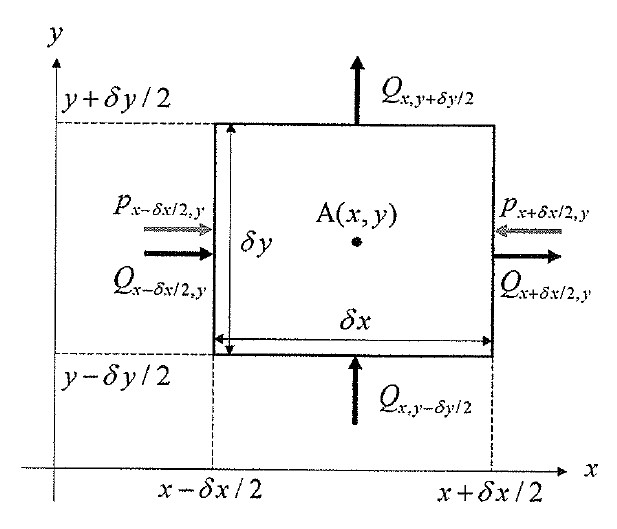
\includegraphics[width=120mm]{images/continuity_equation.jpg}
        \caption{R3 試験問題[7]}
    \end{center}
\end{figure}
\subsubsection{2次元の連続の式の導出}
\begin{itembox}[l]{Point}
    \begin{center}
        時刻$t-\delta t/2\leq t \leq t+\delta t/2$の微小時間$\delta t$間の流れについて\textgt{空間}・\textgt{時間}の観点から保存則を立てる!!
    \end{center}
\end{itembox}
図1において、連続の式を導出する。
\noindent$\delta t$間に流入する流体の質量を$M_{in}$、$\delta t$間に流出する流体の質量を$M_{out}$、$\delta t$間の質量増加量を$\Delta M$とすると、\\
・\textgt{流入・流出量(空間的観点)}
\begin{eqnarray*}
    M_{in}&=&\left(\rho u\right)_{x-\frac{1}{2}\delta x}\delta y \delta t+\left(\rho v\right)_{y-\frac{1}{2}\delta y}\delta x \delta t\\
    M_{out}&=&\left(\rho u\right)_{x+\frac{1}{2}\delta x}\delta y \delta t+\left(\rho v\right)_{y+\frac{1}{2}\delta y}\delta x \delta t\\
\end{eqnarray*}
\noindent
・\textgt{質量増加量(時間的観点)}
\begin{eqnarray*}
    \Delta M=\left(\rho\right)_{t+\frac{1}{2}\delta t}\delta x \delta y-\left(\rho\right)_{t-\frac{1}{2}\delta t}\delta x \delta y
\end{eqnarray*}
質量保存則より、
\begin{eqnarray*}
    (質量増加量)&=&(流入量)-(流出量)\\
    \Delta M&=&\quad M_{in}\quad -\quad M_{out}\\
\end{eqnarray*}
※ 「増加量」は「流入量」$\geq$「流出量」のときに増加する\\
\\
ここで、$\delta x, \delta y, \delta t$のオーダまでTaylor級数展開すると\\
\\
※ ここでは、点$(x,y)$周りの$\left(x,y\right)=\left(x\pm \frac{\delta x}{2},y\pm \frac{\delta y}{2}\right)$のときについて考えている。
\begin{eqnarray*}
    \left(\rho u\right)_{x\pm \frac{1}{2}\delta x}&=&\rho u\pm \frac{\delta x}{2}\frac{\partial\left(\rho u\right)}{\partial x}+O\left(\delta x^2\right)\\
    \left(\rho v\right)_{y\pm \frac{1}{2}\delta y}&=&\rho v\pm \frac{\delta y}{2}\frac{\partial\left(\rho v\right)}{\partial y}+O\left(\delta y^2\right)\\
    \left(\rho\right)_{t\pm \frac{1}{2}\delta t}&=&\rho \pm \frac{\delta t}{2}\frac{\partial \rho}{\partial t}+O\left(\delta t^2\right)
\end{eqnarray*}
したがって、上式を代入すると、
\begin{eqnarray*}
    \dfrac{\partial \rho}{\partial t}\delta x \delta y \delta t&=&-\left(\frac{\partial\left(\rho u\right)}{\partial x}+\frac{\partial\left(\rho v\right)}{\partial y}\right)\delta x \delta y \delta t\\
\end{eqnarray*}
これを変形して、
\begin{eqnarray*}
    \dfrac{\partial p}{\partial t}+\frac{\partial\left(\rho u\right)}{\partial x}+\frac{\partial\left(\rho v\right)}{\partial y}&=&0
\end{eqnarray*}
以上より、2次元空間における連続の式を導くことができた。
\subsubsection{2次元のオイラーの運動方程式の導出}
\begin{itembox}[l]{Point}
    \begin{center}
        \textgt{ニュートンの第二法則}\quad$F=ma$を流体について立てる!!
    \end{center}
\end{itembox}
\textgt{($x$方向)}\\
・\textgt{流体の質量:$m$}\\
\begin{eqnarray*}
    m=\rho \delta x \delta y
\end{eqnarray*}
・\textgt{加速度:$a$}\\
$x$方向の速度$u$の全微分$du$は、
\begin{eqnarray*}
    du=\dfrac{\partial u}{\partial x}dx+\dfrac{\partial u}{\partial y}dy+\dfrac{\partial u}{\partial t}dt
\end{eqnarray*}
\subsection{流体のせん断応力}
流体の流れに平行な軸を$x$軸、垂直な軸を$y$とすると,せん断応力$\tau\left(y\right)$は以下のように表せる。
\begin{itembox}[l]{せん断応力(2次元)}
    \begin{eqnarray*}
        \tau\left(y\right)=\dfrac{du}{dy}
    \end{eqnarray*}
\end{itembox}
\subsection{レイノルズ数}
\begin{itembox}[l]{レイノルズ数}
    \begin{eqnarray*}
        \mathrm{Re}&=&\dfrac{UL}{\nu}\\
        \mathrm{Re} &:& レイノルズ数\\
        U &:& 代表速度\\
        L &:& 代表長さ\\
        \nu &:& 動粘性係数
    \end{eqnarray*}
\end{itembox}
\subsection{流れ関数}
\subsection{速度ポテンシャル}
\end{document}